% Generated from existing finite data; ALG-NS-LOWER, ALG-DEGREE-CURVES, ALG-PC-ALPHA-GROUPING.
\section{Degree results and finite computation evidence}
\label{sec:degrees}
For the actual full-count calibration over $\mathbb Q$, the compiled lower
theorem applies to every supplied ordinary certificate. Here $A$ is the
multiplier of the single count constraint $\sum_iX_i-\pi(N)$, not an arbitrary
family multiplier $A_j$:
\[
 \deg A\geq\alpha(N),\qquad
 \deg\bigl(A(\textstyle\sum_i X_i-\pi(N))\bigr)\geq\alpha(N)+1,
 \qquad \alpha(N)=\pi(N)-r(N).
\]
The required degree is unbounded along even $N$. Neither theorem asserts
the existence of a certificate. Equality is established by existing exact
finite arithmetic only at the $26$ measured even points $N=10,12,\ldots,60$:
the rational identities and the finite-field minima both equal $\alpha+1$,
with degrees between $3$ and $14$. This finite tightness is not a compiled
universal upper theorem. The universal upper construction with midpoint
loops remains blocked; its no-loop counterpart has only paper status.
\ev{ALG-NS-LOWER}\ev{ALG-NS-UPPER-LIMIT}\ev{ALG-DEGREE-CURVES}

Polynomial calculus is measured separately, with genuine ordinary powers,
input rules, binary linear combinations and single-variable multiplication.
The saved measurements over $\mathbb F_{1000000007}$ have exact degrees
$3,3,3,3,4,4,4,4,4,5,5$ for even $N=10,\ldots,30$;
the rational measurements agree at those $11$ points.
The additional finite-field-only points $N=32,34,36$ have degrees $6,5,5$.
All these computations are labeled \textsc{Evidence}; they are not Lean
computations, rational transfers from the larger points, or asymptotic bounds.
The full degree rows are recorded in the publication JSON and Appendix A.
\ev{ALG-DEGREE-CURVES}

\begin{figure}[htbp]
\centering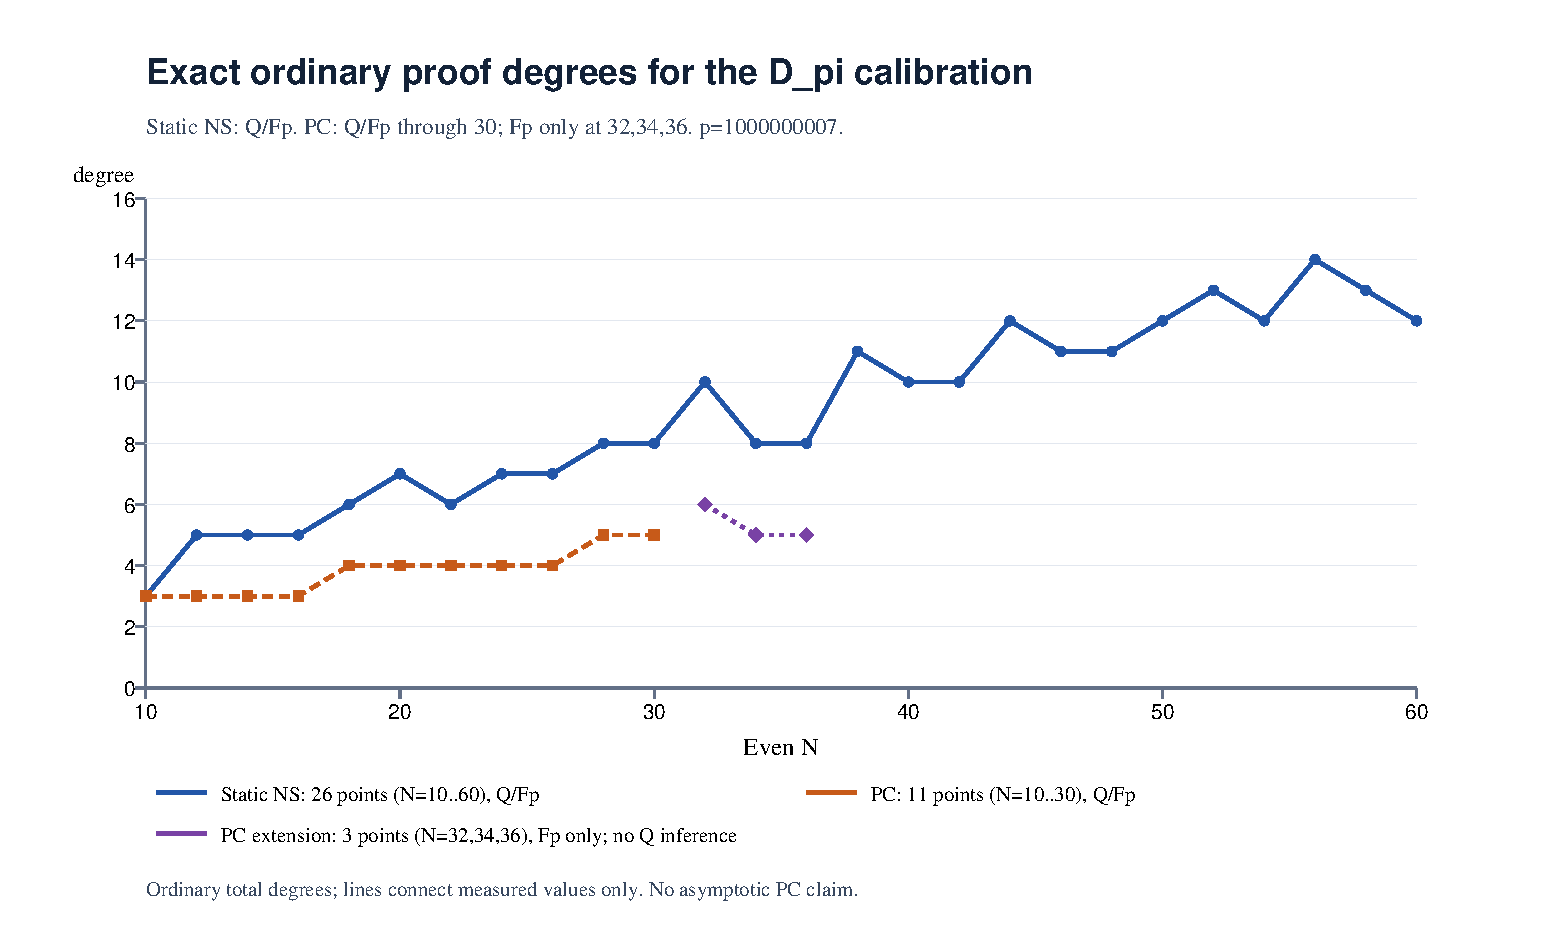
\includegraphics[width=.88\linewidth]{figures/degree_curve.pdf}
\caption{Existing finite degree plot. Static NS equality is measured over
$\mathbb Q$ and $\mathbb F_{1000000007}$ at even $N=10,\ldots,60$.
PC degrees agree over both fields at even $N=10,\ldots,30$; the points
$N=32,34,36$ are finite-field-only. The plot is evidence at these inputs,
not a universal upper bound or a rational transfer.\ev{ALG-DEGREE-FIGURE}}
\label{fig:degree}
\end{figure}

Grouping the existing CSV rows using $\alpha$ from the saved lower-bound
JSON finds the same PC degree whenever $\alpha$ repeats in these $14$
finite-field points. The complete observed groups are:
\begin{center}
\begin{tabular}{@{}lll@{}}
\toprule
$\alpha$ & $N$ & Observed PC degree\\
\midrule
$2$ & $10$ & $3$ \\
$4$ & $12,14,16$ & $3$ \\
$5$ & $18,22$ & $4$ \\
$6$ & $20,24,26$ & $4$ \\
$7$ & $28,30,34,36$ & $5$ \\
$9$ & $32$ & $6$ \\
\bottomrule
\end{tabular}
\end{center}
This is finite group consistency, not a universal dependence theorem or a
closed PC degree formula.\ev{ALG-PC-ALPHA-GROUPING}

The compiled ordinary-Q restriction sends a supplied $D_\pi$ PC refutation
to a genuine Boolean-knapsack refutation on $\alpha$ variables without
increasing ordinary line degree. The explicit external predicate
\texttt{KnapsackLowerBound} remains a hypothesis of its lower corollary.
That conditional corollary is out of scope and is recorded in Appendix B;
the partial lattice, coefficient and count-action lemmas do not remove
the hypothesis.\ev{ALG-PC-HYPOTHESIS}
